Developing retrieval-augmented generation systems is a challenging task that often requires multiple reconfiguration phases \cite{Simon.10112024}. Because RAG systems can involve complex pipelines with iterative or recursive processes, component evaluation and in-depth failure analysis are crucial for tuning the appropriate components. Failures can occur throughout the RAG system as highlighted by Barnett et al. \cite{Barnett.2024}. Since every additional component can influence overall performance, it is indispensable for a robust evaluation framework to assess individual components alongside end-to-end system results. This chapter addresses these challenges by first introducing a validation-test split for evaluation data and justifying its importance. Subsequently, we explore accurate RAG evaluation from two perspectives: end-to-end and component-level assessment. We then delve into methods for accelerating RAG development while ensuring transparent and reproducible results, including Haystack's approach to modular development via configuration files, extended here to support multi-configuration testing. Finally, we cover failure analysis using tracing and the estimation of generalization error.

\section{Validation-Test Split}\label{sec:valtestsplit}
Typical machine learning projects require researchers to collect, prepare, and split data into training, validation, and test sets. This split is crucial for optimizing a model using the training and validation datasets, and subsequently testing its generalization error on the unseen test dataset. The necessity for this process stems not solely from training itself but primarily from tuning models to a given dataset - often involving numerous free parameters (hyperparameters). Whenever tuning parameters based on performance on a specific dataset, it is essential to ensure that the model does not overfit this data. We argue that this challenge is equally present in the development of RAG systems.

Whether training a classifier or configuring a RAG system, both processes involve a large number of free parameters. A RAG system can have hundreds to thousands of them, especially when considering choices for generator models, embedding techniques, corpus content, or system architectures as (indirect) free parameters. Therefore, it is crucial to ensure that the final system configuration is not overfitted to the specific evaluation dataset used during development.

In this framework, we address this by splitting any given evaluation dataset via random sampling into two parts: a validation dataset and a test dataset. We then proceed with evaluation and reconfiguration using \textit{only} the validation dataset, holding out the test data completely until a satisfactory configuration is achieved through iterative refinement. Once the reconfiguration phase is complete, we use the test set \textit{once} to assess whether the performance observed on the validation set generalizes, typically by comparing the validation error (or other metrics) with the test error. The next section explains how RAG systems should be evaluated to maximize their overall performance using this approach. If the validation error is, for some metrics, significantly lower than the test error, then there is a chance of overfitting. We do not perform hypothesis tests within our framework.

\section{Evaluation Techniques}

Evaluating retrieval-augmented generation systems is a challenging task and an active area of research. It inherits common machine learning evaluation challenges, such as data shifts, generalization errors, and data contamination, but also introduces unique failure points due to the complexity of its multi-component design. In this section, we will discuss major failure points specific to RAG systems and explain how this framework aids in their identification. The ultimate goal when tuning a RAG system is to maximize its performance in end-to-end evaluation, ensuring that the system's responses fully and correctly answer user questions or complete assigned tasks.

However, relying solely on end-to-end evaluation makes it difficult to pinpoint which parameters to tune or which data modifications are needed to achieve performance improvements. Figure \ref{fig:failures} illustrates example failures for components in a specific RAG pipeline, but in practice, the potential points of failure are far more numerous. RAG systems operate like complex processing pipelines; identifying and replacing underperforming bottleneck components with more effective ones is essential for optimization. This necessitates rigorous failure analysis. Therefore, every experiment should incorporate tracing mechanisms to track the flow of information and understand the root causes when a query is answered incorrectly. In this framework, we utilize Langfuse's \cite{Langfuse} self-hosted version for tracing. We visualize all metrics and RAG parameters using MLflow \cite{MLflow}. While MLflow also offers tracing and GenAI evaluation modules, we currently opted against using them because its tracing module lacks compatibility with Haystack at present, and its GenAI features require ground-truth documents (which can be impractical, e.g., due to dynamic chunking strategies), are marked as experimental, and are incompatible with our validation-test split methodology.

\begin{figure}
  \centering
  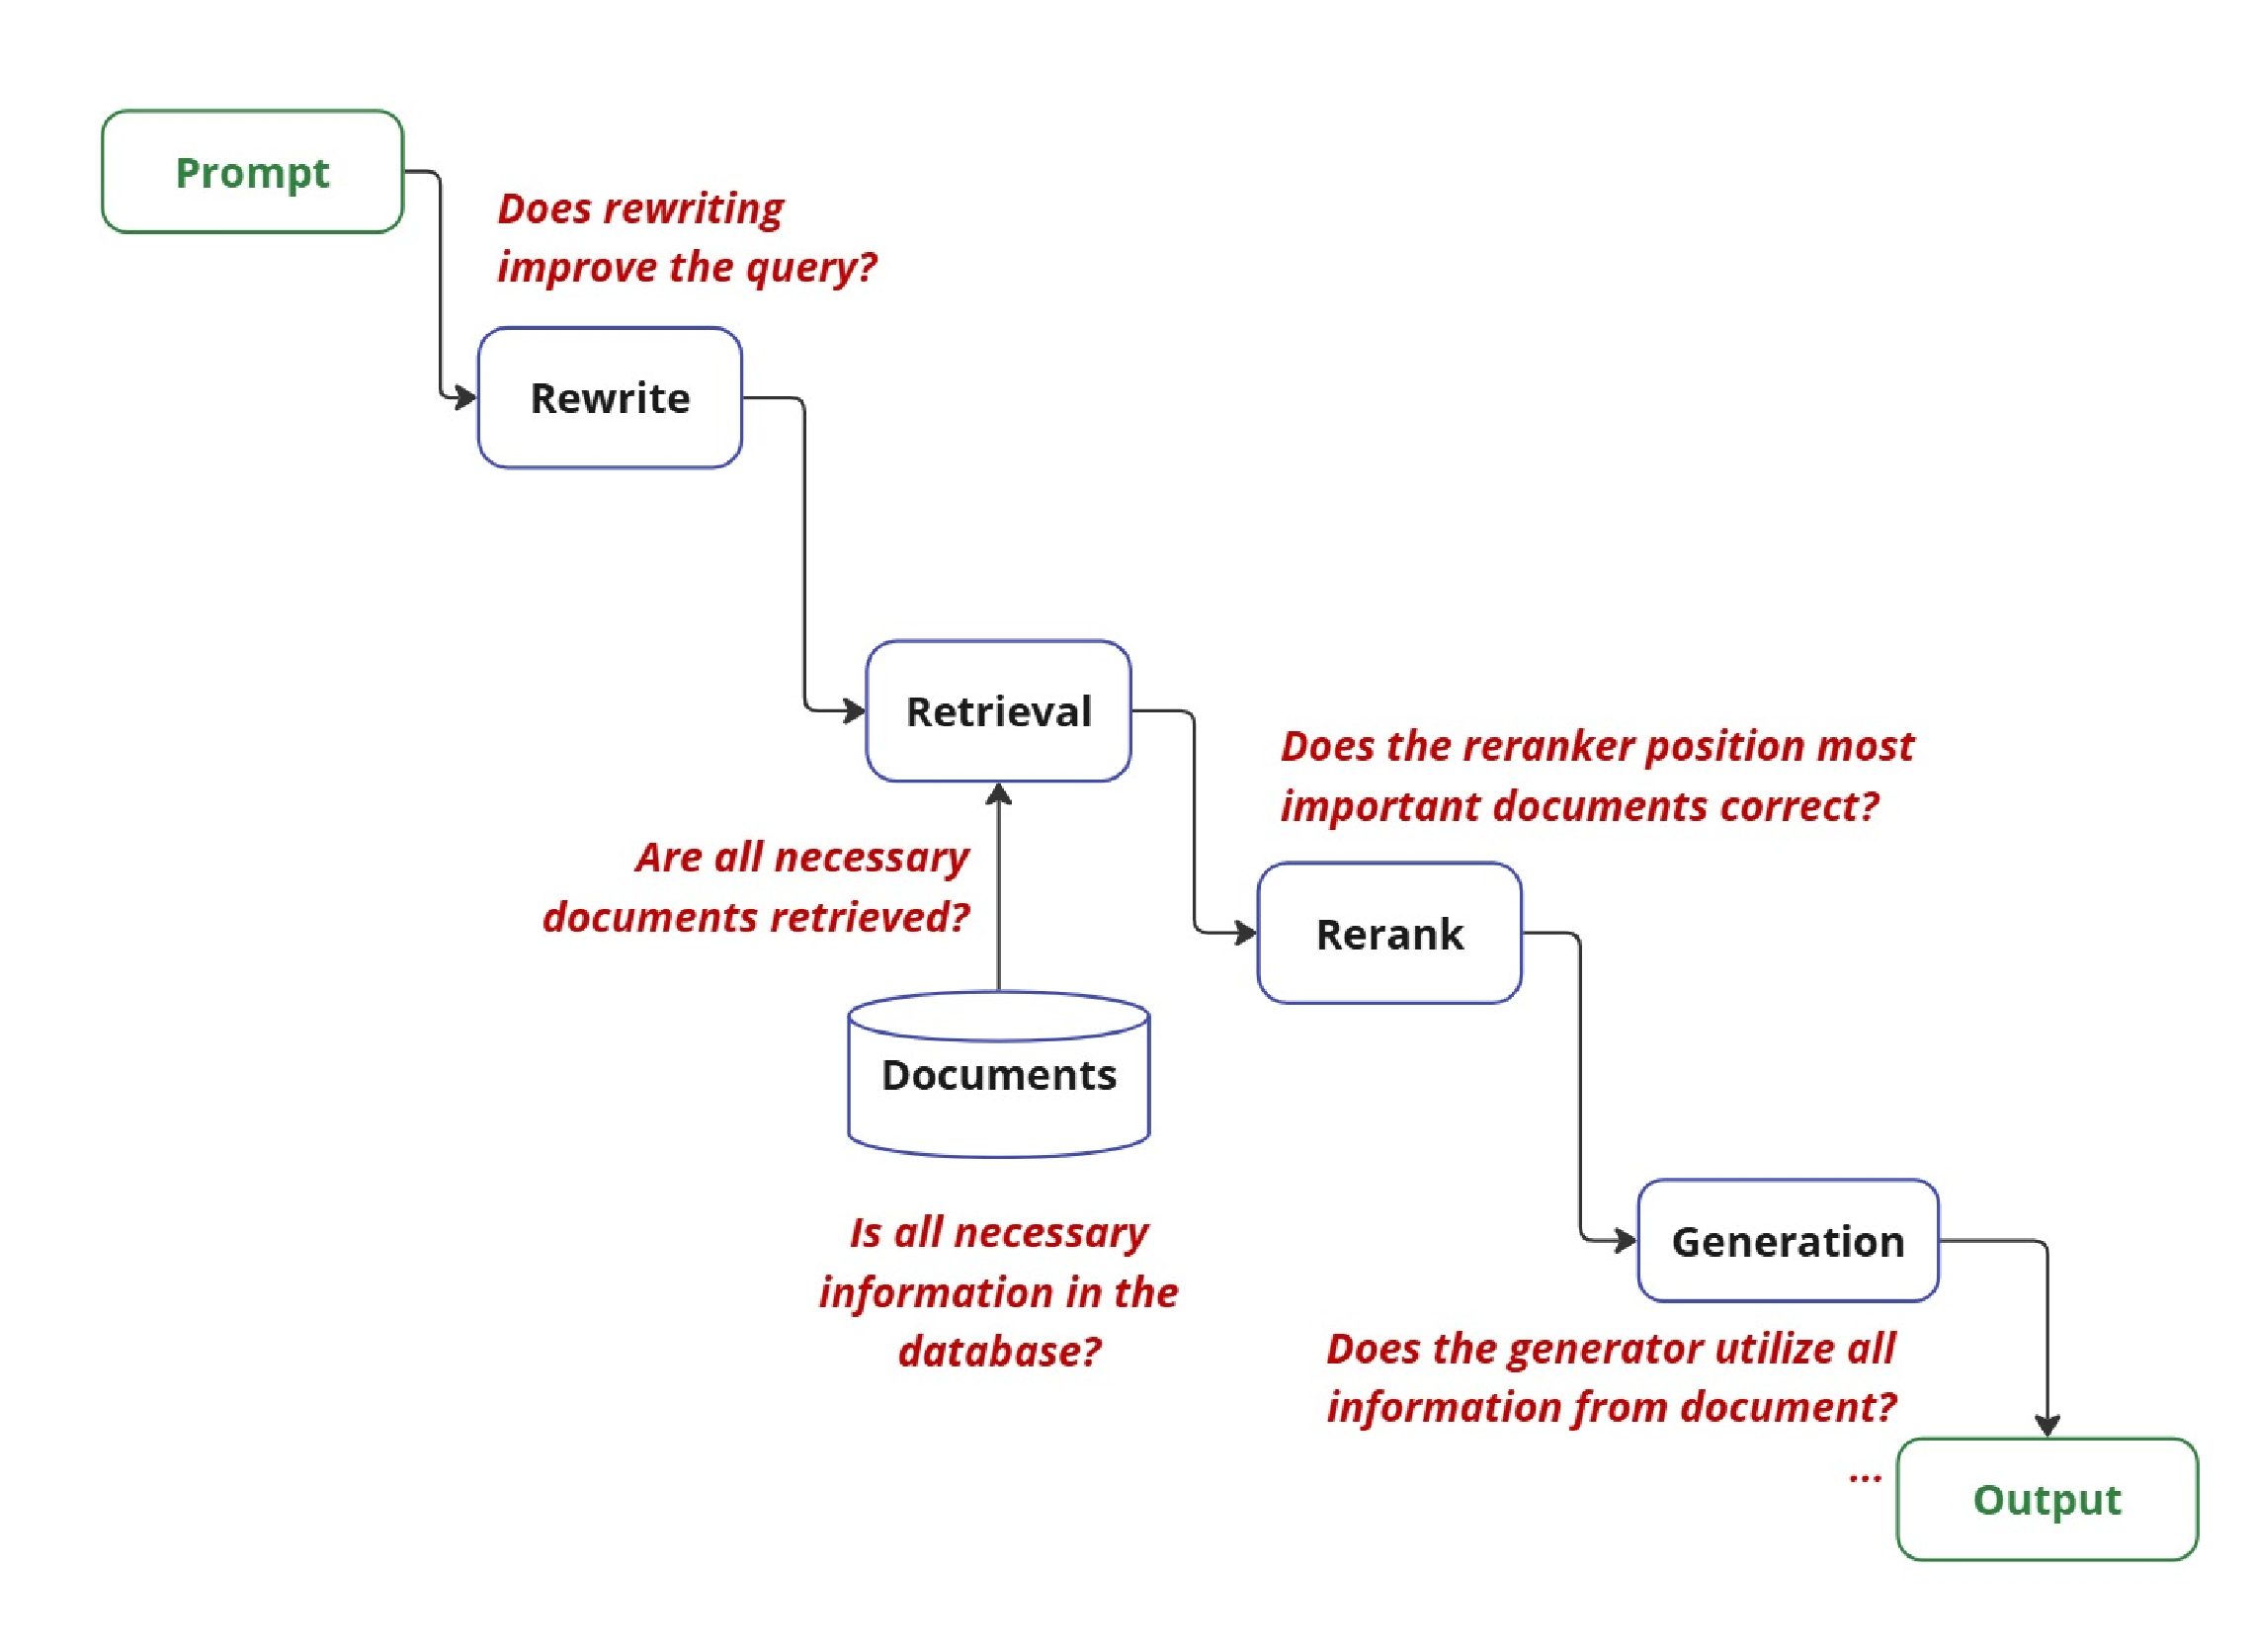
\includegraphics[width=\textwidth]{images/FailurePointExamples.pdf}
  \caption{A RAG pipeline with one failure example for each used component.}
  \label{fig:failures}
\end{figure}

\subsection{End-to-End Evaluation}\label{sec:e2e}

We define end-to-end evaluation as metrics that use the system's input query and its final output, comparing this output against a ground-truth reference to determine correctness. Evaluations that assess intermediate steps, such as retrieval performance or the generator's ability to utilize provided context, are considered component-level evaluations and are distinct from the end-to-end perspective discussed here. In this thesis, our focus is primarily on classification tasks; therefore, the end-to-end metrics employed are limited to those suitable for classification.

{\renewcommand{\arraystretch}{1.5}%
\begin{table}
  \centering
 \begin{tabular}{|l|l|}
  \hline
  \textbf{Metric} & \textbf{Formula / Description} \\[3pt]
  \hline Accuracy & $\frac{TP + TN}{TP + TN + FP + FN}$\\[5pt]
  \hline Precision & $\frac{TP}{TP + FP}$\\[5pt]
  \hline Recall & $\frac{TP}{TP + FN}$\\[2pt]
  \hline F1-Score & $2 \times \frac{Precision \times Recall}{Precision + Recall}$\\[2pt]
  \hline Matthews Correlation & $\frac{TP \times TN - FP \times FN}{\sqrt{(TP + FP)(TP + FN)(TN + FP)(TN + FN)}}$\\Coefficient & \\[2pt]
  \hline False-Positive Rate & $\frac{FP}{FP + TN}$\\[2pt]
  \hline False-Negative Rate & $\frac{FN}{FN + TP}$\\[2pt]
  \hline
 \end{tabular}
 \caption{Typical classification metrics used for experiments involving RAGs or LLMs\cite{Hou.8212023,Zeng.28.03.2024}.}
 \label{table:classification_metrics}
\end{table}}

In stark contrast to evaluating open-ended generative tasks, classification tasks benefit from well-established metrics and evaluation methods. Table \ref{table:classification_metrics} presents commonly used classification metrics relevant for RAG and LLM experimentation.

Meaningful end-to-end evaluation requires researchers to establish \textit{baselines} for their experiments. Baselines make results interpretable by providing essential points of comparison. Therefore, this framework implements two default baselines used when initiating an experiment. The first baseline consists solely of a standalone LLM answering the query without retrieval. The second is a naive RAG system employing BM25 retrieval with data from the predefined corpus (a simple Retrieve-Read pipeline, cf. Section \ref{sec:naive_rags}). The standalone LLM baseline helps justify the complexity overhead of implementing a RAG system; if an evaluated RAG system cannot surpass the performance of the LLM baseline, a simpler approach might be preferable. Advanced RAG systems often involve more components, potentially leading to longer computation times and increased costs. Outperforming the naive RAG baseline demonstrates the value added by the more advanced RAG configuration beyond simple keyword retrieval.

\begin{figure}[!ht]
  \centering
  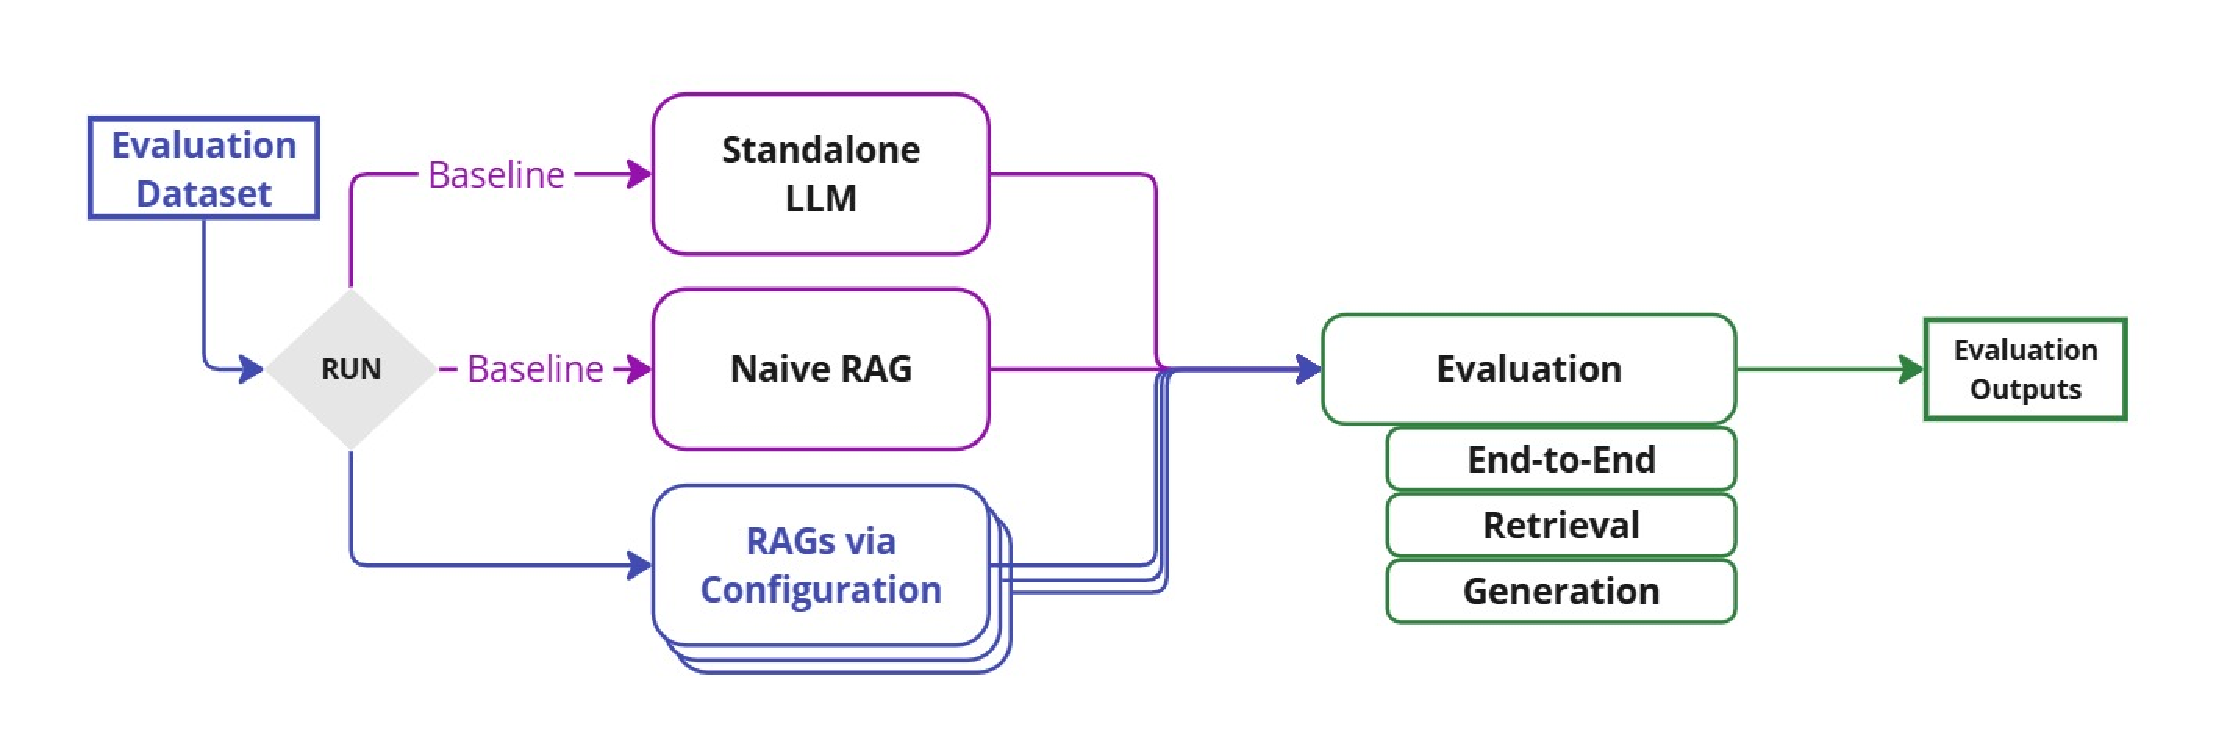
\includegraphics[width=\textwidth]{images/FrameworkBaselines.pdf}
  \caption{Framework Overview: Researchers define configuration files for RAG variations, which are evaluated against the standalone LLM and naive RAG baselines using end-to-end metrics.}
  \label{fig:framework-baselines}
\end{figure}
% \cite{Ru.15.08.2024.} Eventhough all components of a RAG-system affect its overall performance, there are ones that can not be evaluated directly.  \\

Figure \ref{fig:framework-baselines} illustrates the state of our framework as defined thus far and clarifies our approach. It depicts the process where evaluation data is used to compute metrics for both the defined baselines and the RAG configurations under test, performing both end-to-end and component-wise (retrieval and generation) evaluations. The following section details the component evaluation methodology employed in our framework.

\subsection{Component Evaluation}

Component evaluation is necessary to detect performance bottlenecks or issues introduced by individual components or problematic interactions between them \cite{Salemi.2024}. In Figure \ref{fig:failures}, we presented a few examples of such failures. While illustrative, this is far from an exhaustive list of potential failure points in a complex RAG system. We argue that potentially *all* components, no matter how seemingly small their impact, can contribute significantly to the overall system's failure rate. Therefore, ideally, it would be necessary to evaluate them all component-wise.

However, current literature on component evaluation primarily focuses on the core retrieval and generation (\textit{read}) stages. Furthermore, we want to emphasize that evaluating components in complete isolation from others is often impractical. If, for example, one wished to evaluate the generator component independently of the retrieval step, it would require providing a ground-truth dataset of ideal retrieved contexts for each query. This might be feasible for simple scenarios requiring only a single, easily identifiable document chunk (e.g., a sentence providing a direct answer). Yet, real-world scenarios frequently involve more complex cases, such as ambiguous queries, multifaceted questions requiring information synthesis, or queries that do not require retrieval at all \cite{Huang_2023}. Furthermore, if the researcher modifies the chunking strategy (e.g., size or technique), the ground-truth contexts would need to be recreated, as the previously selected chunks might no longer exist (cf. Section \ref{sec:advanced_rags}).

Considering other components besides the retriever, such as query rewriters or document rerankers, establishing ground-truth data becomes even more problematic. The purpose of rewriting a query, for instance, is often to improve subsequent retrieval performance. Thus, its effectiveness is inherently dependent on the specific retriever used and cannot easily be assessed against fixed, retriever-agnostic ground-truth examples in an evaluation dataset.

Given these challenges, the primary purpose of component evaluation shifts towards identifying weaknesses within the RAG pipeline rather than achieving perfect isolated assessment. It is often more feasible to evaluate the RAG system using only the initial inputs and final ground-truth answers for end-to-end metrics, while employing non-deterministic LLM-as-a-Judge methods for assessing intermediate steps where appropriate. The LLM-as-a-Judge approach involves using a powerful LLM (often significantly larger or specifically trained for evaluation) to assess the quality of intermediate outputs (such as retrieved context relevance) or final responses \cite{Chiang.2023}. Instead of relying solely on numerical metrics, the judge LLM provides qualitative assessments or scores based on predefined criteria.

Relying primarily on system input and final ground-truth datasets for evaluation offers significant time savings compared to creating extensive intermediate ground truths. However, detailed failure analysis to pinpoint the root cause of errors still necessitates tracing individual pipeline executions, which we utilize in this framework with Langfuse. The following sections detail our approach to evaluating the key retrieval and generation blocks using a combination of these techniques.

\paragraph{Retrieve}
Evaluating the retrieval component is arguably one of the most challenging aspects of RAG assessment for several reasons. First, retrieving more documents does not necessarily imply better final results, and it is often unclear which specific set of documents will best enable the generator to produce the optimal answer \cite{Jin.5222024}. Second, real-world indexed corpora often contain redundant and contradictory information \cite{Yu.2024}. Third, some queries require retrieving diverse perspectives on a topic, highlighting various considerations. Fourth, the quality of the input query itself significantly affects retrieval performance; queries can be overly complex or ambiguous, or may not even require retrieval, potentially leading to generator hallucinations if irrelevant or misleading context is fetched \cite{Huang_2023, Mallen.2022}.

While retrieved documents can often be assessed in a binary fashion (relevant/irrelevant), allowing for metrics based on \textit{True/False Positives/Negatives}, simple metrics like precision and recall are often not sufficiently sensitive to capture nuanced differences in retrieval quality \cite{Yu.2024}. There is a clear need for evaluation techniques that also consider the ranking of retrieved documents.

Furthermore, significant limitations exist when working with ground-truth data for retrieval evaluation. Defining a definitive ground-truth set of relevant context documents for a given query can be ambiguous and challenging even for human experts, although LLM-as-a-Judge models have shown high correlation with human judgments in this area \cite{Chiang.2023}. Compounding this issue is the dynamic nature of chunking during reconfiguration. Every time a chunking technique or parameter is altered, the resulting indexed documents change, necessitating the recreation of ground-truth retrieval datasets. This poses a significant bottleneck for rapid development cycles, yet tuning chunking strategies is crucial. Therefore, to maintain flexibility and speed, this framework focuses primarily on LLM-as-a-Judge evaluation for the retrieval component, particularly enabling effective chunking parameter tuning.

We utilize a metric named \textit{Context Relevance} (akin to \textit{Context Precision} in other frameworks) which employs an LLM-as-a-Judge. This metric assesses the relevance of each retrieved document concerning the input query. A binary approach is typically adopted: the LLM-as-a-Judge determines if a document contains statements relevant to the query. If yes, the document scores 1 (relevant); otherwise, it scores 0 (irrelevant). Haystack's `ContextRelevanceEvaluator` \cite{Pietsch_Haystack_the_end-to-end_2019}, for instance, implements such a binary assessment. The final \textit{Context Relevance} score is the mean of these binary scores across all retrieved documents for a query (and typically averaged over all queries in the dataset), yielding a score analogous to Mean Precision. While some frameworks like RAGAS might infer retrieval quality from the generated response, our approach, similar to Haystack's, directly evaluates the relevance of the retrieved documents themselves via the LLM-as-a-Judge.

Recognizing that simple relevance counts (like Context Relevance/Precision) do not capture ranking quality, we also implement \textit{Mean Average Precision at K (MAP@K)} to offer a complementary, rank-aware perspective. MAP@K evaluates whether relevant documents are ranked higher in the retrieved list \cite{EvidentlyAIInc..25.02.2025}. 

$$MAP@K=\frac{1}{|Q|}\sum_{q=1}^{|Q|}AP@K$$
$$AP@K=\frac{1}{N}\sum_{k=1}^{K}Precision(k) \cdot rel(k)$$
\begin{itemize}
  \item $|Q|$ is the total number of queries in the evaluation set.
  \item $q$ represents a specific query
  \item $AP@K$ is the Average Precision at K for a specific query.
  \item $N$ is the total number of relevant items for a particular query.
  \item $K$ is the number of top documents being evaluated.
  \item $k$ represents a specific position in the ranked list of retrieved documents.
  \item $Precision(k)$ is the precision calculated at position $k$, defined as the number of relevant items among the top $k$ items divided by $k$.
  \item $rel(k)$ equals 1 if the item at position $k$ is relevant and 0 otherwise.
\end{itemize}

The formula presented is the standard definition of MAP@K \cite{Lin.13.10.2020}. While in some traditional information retrieval scenarios K might be set very high, this can be computationally expensive and may conflict with the goal of providing concise context. Therefore, we calculate MAP@K based on the actual number of documents retrieved (i.e., the system's configured \textit{Top-K} parameter). \textit{Context Relevance} measures overall retrieval quality by focusing on the proportion of relevant items, while \textit{MAP@K} specifically assesses the ranking quality within the retrieved set. A low \textit{Context Relevance} score alongside a high \textit{MAP@K} score might indicate that while relevant documents are found and ranked well, too many irrelevant documents are also being retrieved, suggesting the \textit{Top-K} parameter could potentially be reduced. Conversely, a low \textit{MAP@K} suggests the retrieval/ranking mechanism itself needs adjustment, as irrelevant documents frequently appear high in the results list.

\begin{figure}[!ht]
  \centering
  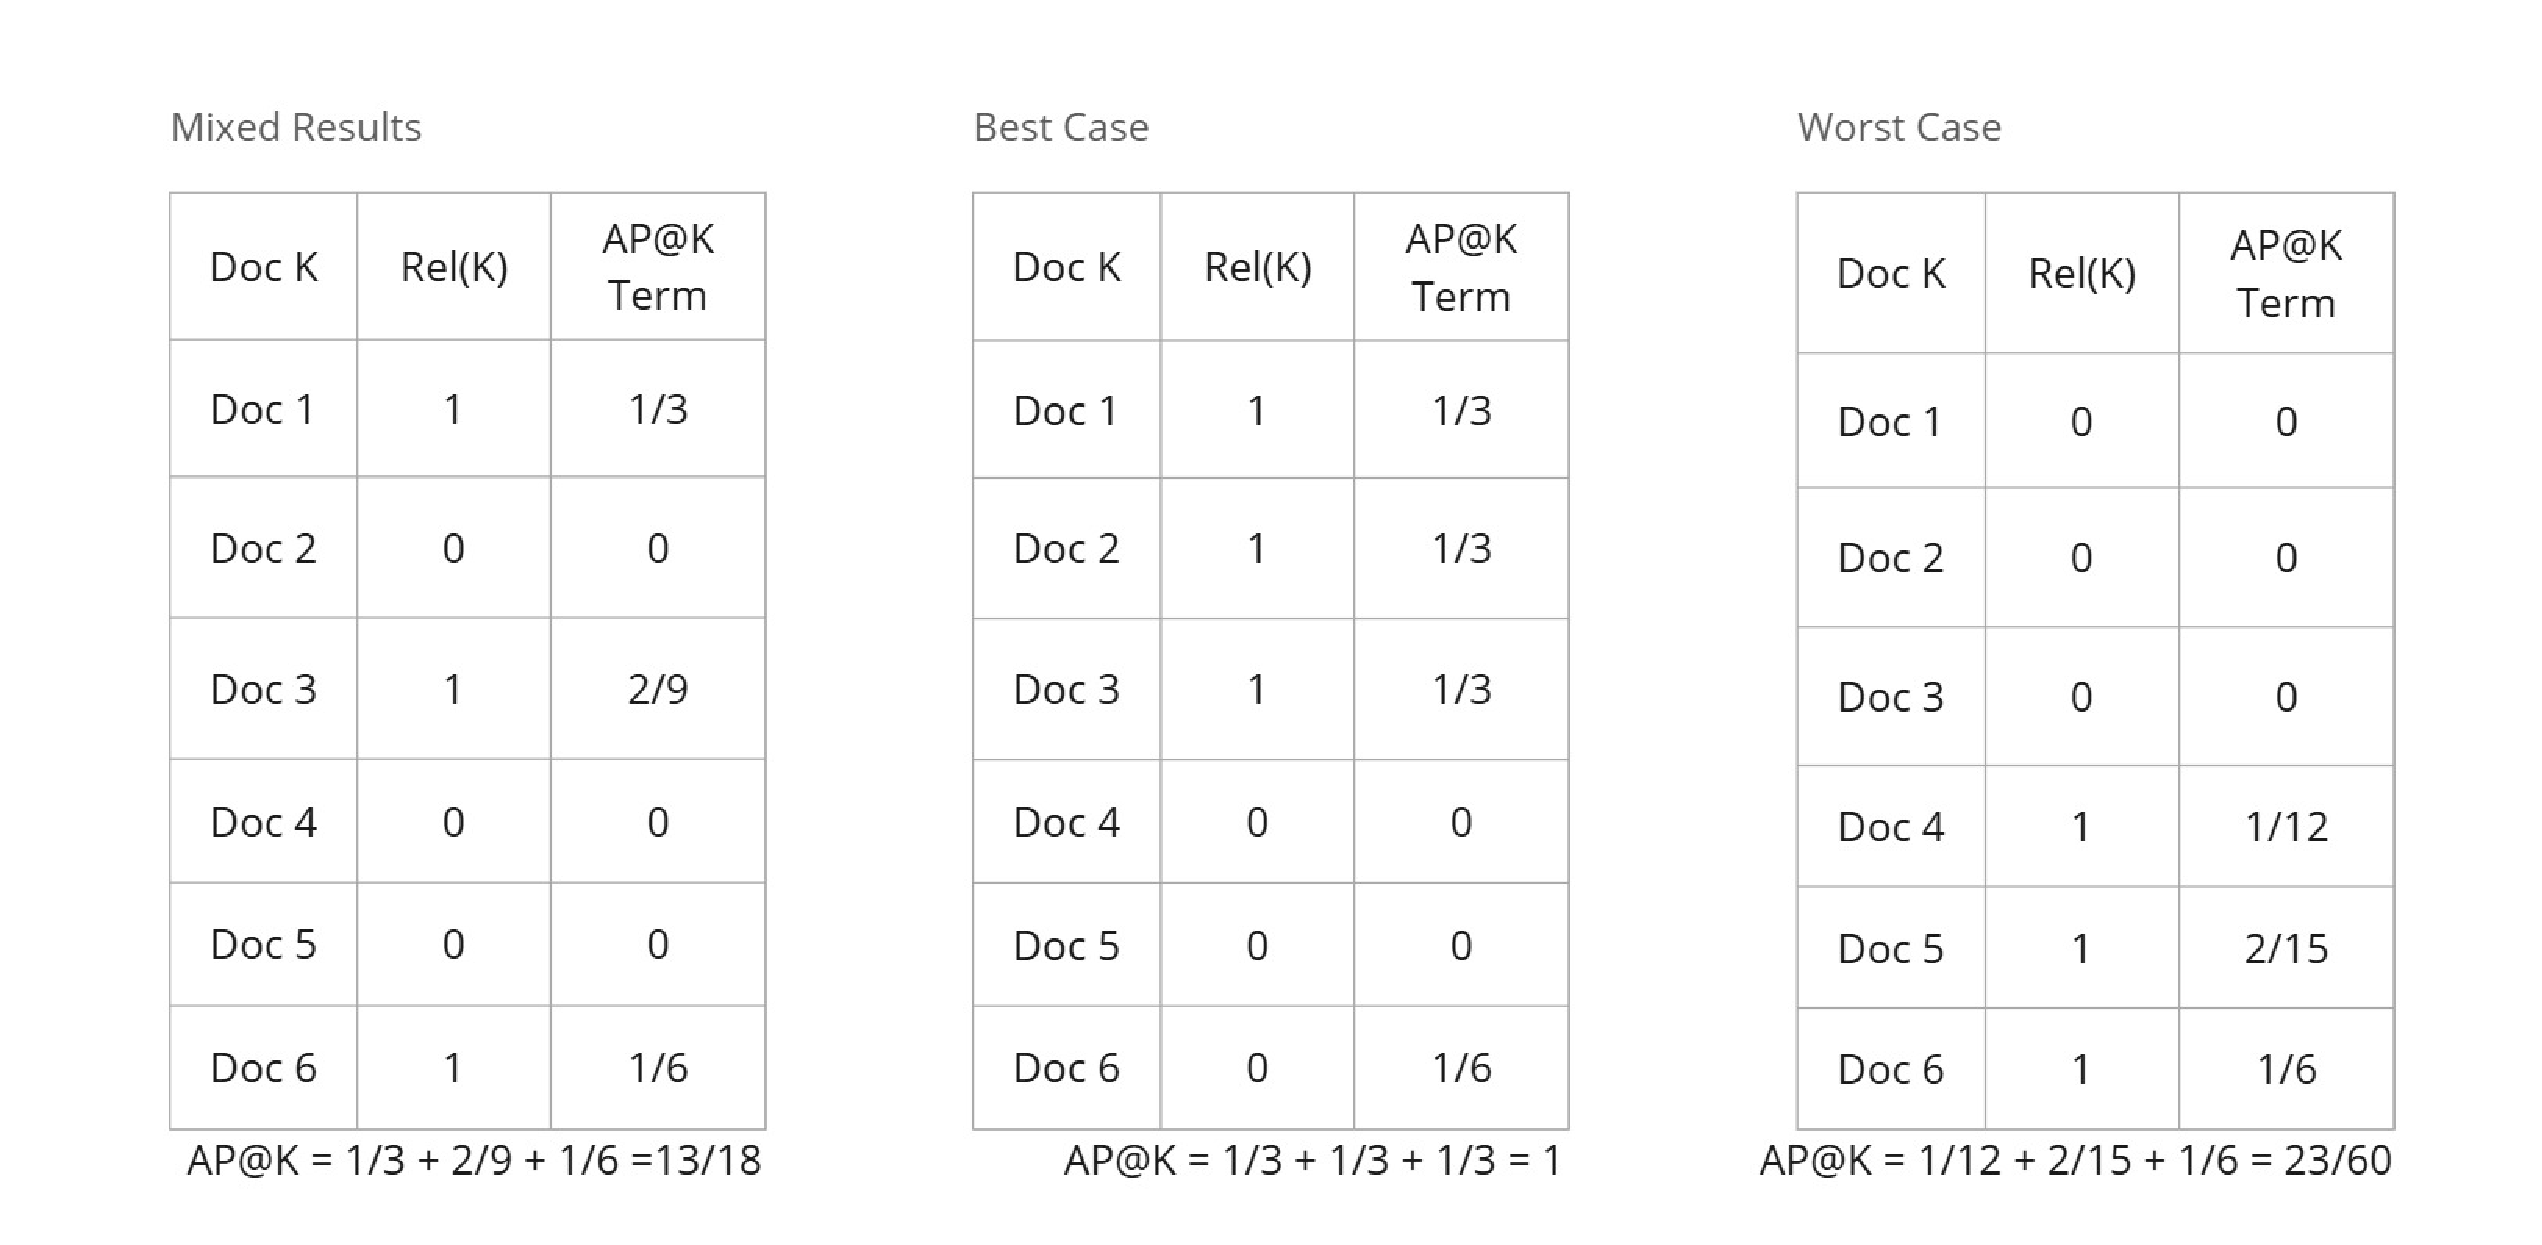
\includegraphics[width=\textwidth]{images/APatK.pdf}
  \caption{An example of the AP@K metric for a single query. For each retrieved document, the relevance and precision from the first to the K-th document are averaged across all retrieved documents.}
  \label{fig:APatK}
\end{figure}


\paragraph{Generators}
Generators in RAG systems, typically based on transformer architectures, were not initially designed primarily for classification tasks. Consequently, ensuring their outputs adhere to specific, desired formats (e.g., producing only \textit{valid} or \textit{invalid}) is an important preliminary check. This necessitates a metric or process to evaluate the generator's ability to follow formatting instructions; we refer to this as \textit{format validation}. However, a significant challenge arises when evaluating generators solely on classification accuracy: simple binary outputs (\textit{True/False}, \textit{Valid/Invalid}) make it difficult, if not impossible, to directly assess crucial underlying aspects like whether the retrieved context was properly utilized or how relevant the generated answer is to the context.

Even when the final prediction is simply \textit{True} or \textit{False}, the underlying generation process involves varying degrees of context utilization and reasoning quality. Therefore, in this framework, we adopt a slightly modified output format for classification tasks to gain more insight. Instead of requiring the generator to produce *only* the binary label (e.g., \textit{0}/\textit{1}, \textit{valid}/\textit{invalid}, \textit{True}/\textit{False}), we prompt it to also output its reasoning *alongside* the classification verdict. The primary technical constraint is that the final answer label itself (e.g., the phrase \textit{'The answer is "True"'}) must be present in a predictable pattern within the output, allowing for its reliable extraction, for instance, using a regular expression for end-to-end metric calculation. Figure \ref{fig:answerreason} shows a simple example.

\begin{figure}[!ht]
  \centering
  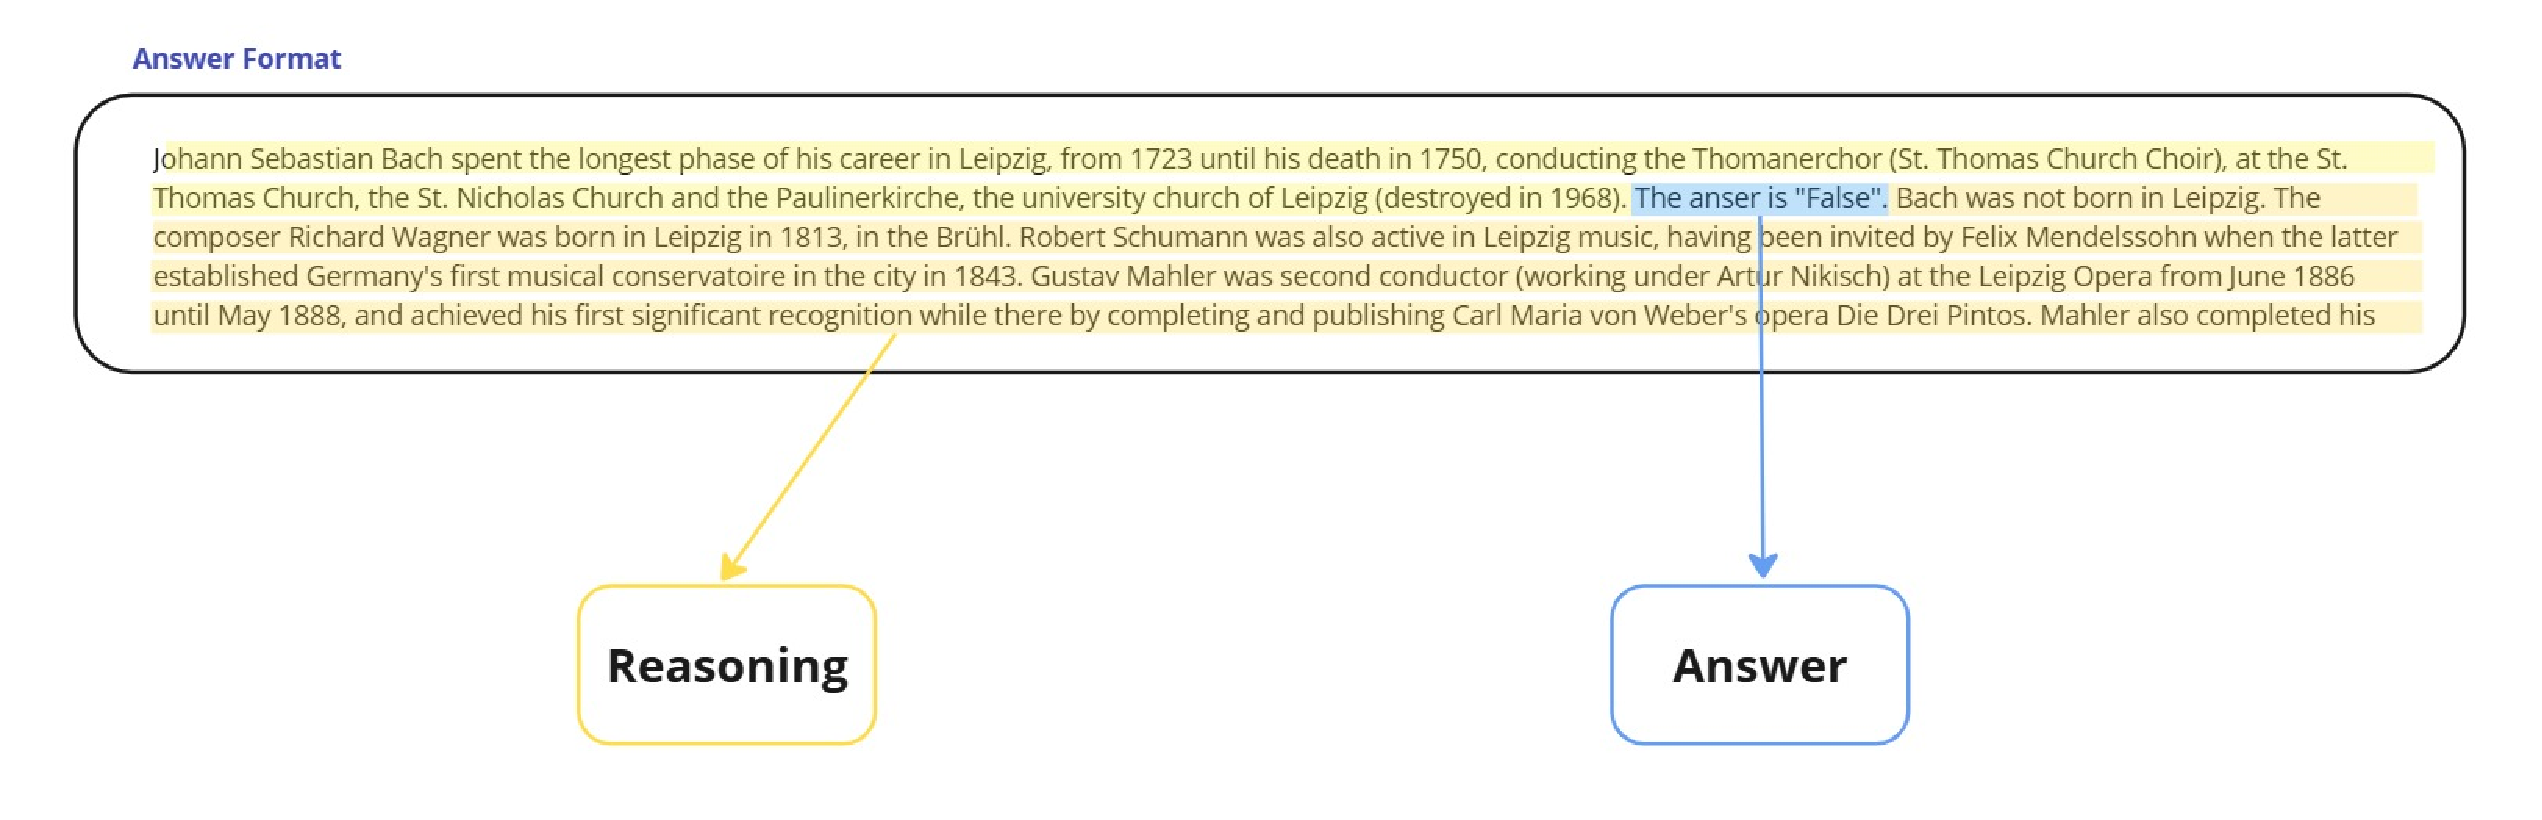
\includegraphics[width=\textwidth]{images/Answer-vs-Reasoning.pdf}
  \caption{Example of a generator's answer, including reasoning, and the final extracted answer used for binary classification.}
  \label{fig:answerreason}
\end{figure}

This approach has several positive side effects. First, the reasoning can be measured to assess context utilization or answer relevance, which is important for debugging the system. If the retrieved context is not sufficiently utilized, this issue might not be identified by analyzing only binary classes. Second, it enables researchers to leverage the current test-time compute paradigm shift for large language models or \textit{large reasoning models}. In practice, these models use \textit{<think>...</think>} tags and various search algorithms to find the optimal reasoning path before answering the query, leading to significantly better results \cite{Xu.16.01.2025}.


\subsection{Component Block Evaluation}

Beyond evaluating individual core components like the retriever and generator, we must also consider components whose performance is highly interdependent or difficult to assess in isolation. Examples in advanced RAG systems include query rewriters and document rerankers. Rewriters aim to optimize the input query for the specific retrieval method and available context. The optimal rewriting strategy often depends on whether the subsequent retriever is sparse (keyword-based) or dense (embedding-based), requiring optimization towards relevant keywords or semantic similarity, respectively. Rerankers, operating post-retrieval, aim to reorder the retrieved documents to prioritize the most relevant or useful ones for the generator.

Both rerankers and generators significantly influence, and rely upon, effective context utilization – the ability to synthesize a coherent and correct answer based on facts within the retrieved context. However, interactions can be complex. For instance, phenomena like 'lost-in-the-middle', where information in the middle of long contexts is less effectively utilized, significantly impact performance, and different LLMs exhibit varying susceptibility to this effect \cite{Liu.06.07.2023}. Consequently, combining the individually 'best' performing reranker and generator (based on isolated metrics) might not yield the optimal system-level result due to potentially incompatible interactions or unforeseen effects on how the generator utilizes the context provided by the reranker. This highlights the need for evaluating interacting components together as functional 'blocks' within the pipeline, rather than relying solely on optimizing components in isolation. Rigorous testing of potential component block configurations becomes essential.

\paragraph{How to evaluate such component blocks?}

\begin{figure}[!ht]
  \centering
  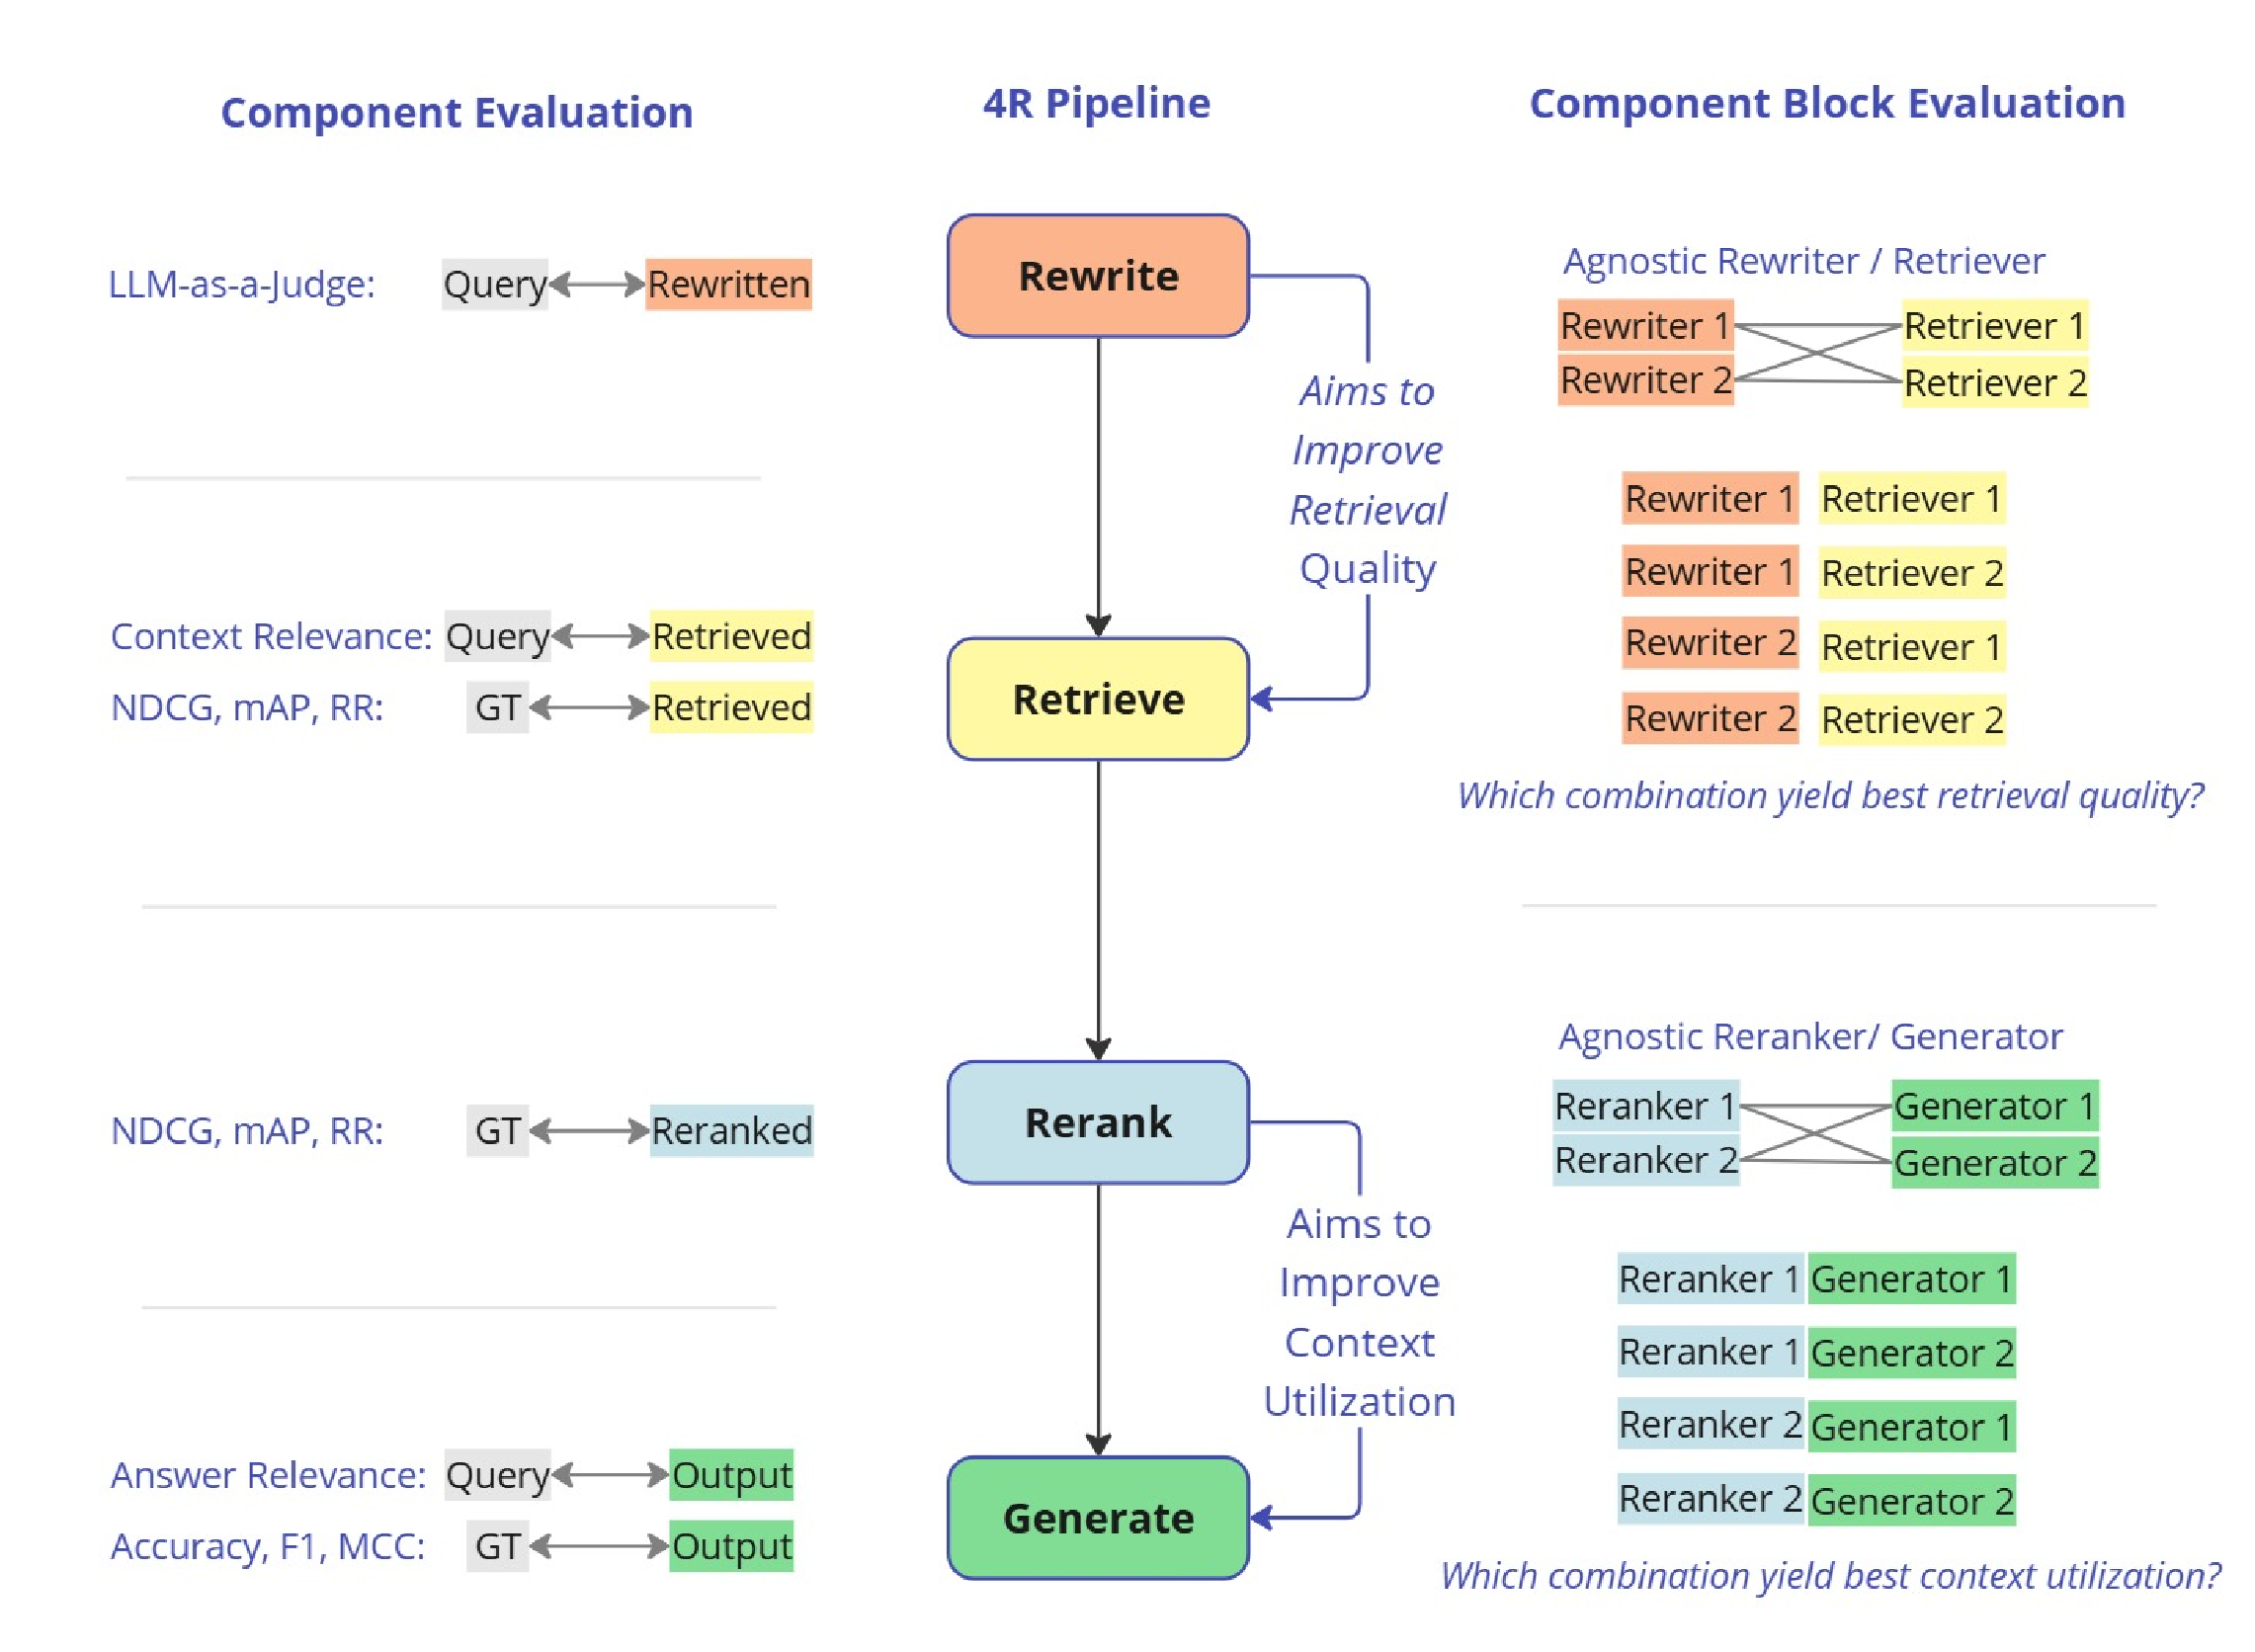
\includegraphics[width=\textwidth]{images/ComponentBlockEvaluation.pdf}
  \caption{Comparison of isolated component evaluation of each component and component block evaluation, where several components with the same goal are evaluated.}
  \label{fig:componentblockeval}
\end{figure}


We can differentiate two major functional blocks where such interactions are common: pre-retrieval and post-retrieval. The evaluation of pre-retrieval component blocks (e.g., involving query rewriters) often relies on observing their impact on subsequent retrieval performance. The primary goal of pre-retrieval steps is typically to enhance retrieval quality, ensuring the retriever finds the necessary documents or chunks for the task. Common pre-retrieval techniques include query routing, query transformation, and query expansion. Additionally, parameters adjusted during the data ingestion stage, such as chunking methods, document selection criteria, and preprocessing steps, also significantly influence subsequent retrieval quality and can be considered part of optimizing the broader pre-retrieval process.

Post-retrieval components, such as rerankers, primarily aim to improve context utilization by the generator. Ideally, the generator receives a concise, curated list of documents tailored to its processing capabilities and the specific query, and rerankers help achieve this by reordering the initially retrieved set. Evaluating the impact of this reranking step is crucial as it directly influences overall system performance. The effectiveness of the reranker block can be assessed using metrics similar to those used for retrieval (e.g., Context Relevance, MAP@K applied to the *reranked* list) or by its downstream impact on end-to-end performance.

Since many components beyond the core retriever and generator lack direct, intrinsic evaluation metrics, their effectiveness must often be assessed indirectly through replacement experiments. In this approach, different variations of a component or block are tested while keeping the rest of the pipeline constant, and the results are compared using relevant block-level or end-to-end metrics. For instance, different rewriter approaches (e.g., using various models, prompting techniques, or alternative components) can be evaluated as distinct variations. The RAG system is then evaluated with each variation. The configuration yielding the best performance on relevant metrics (e.g., end-to-end accuracy or retrieval metrics measured after the combined Rewrite-retrieve steps) is considered superior for that specific pipeline configuration. This comparative evaluation approach necessitates testing multiple RAG variations to enable rigorous assessment. The next section introduces our approach to facilitate such multi-configuration experiments efficiently.

\section{Fast RAG Development}\label{sec:fastrag}

\begin{figure}[!ht]
    \centering
    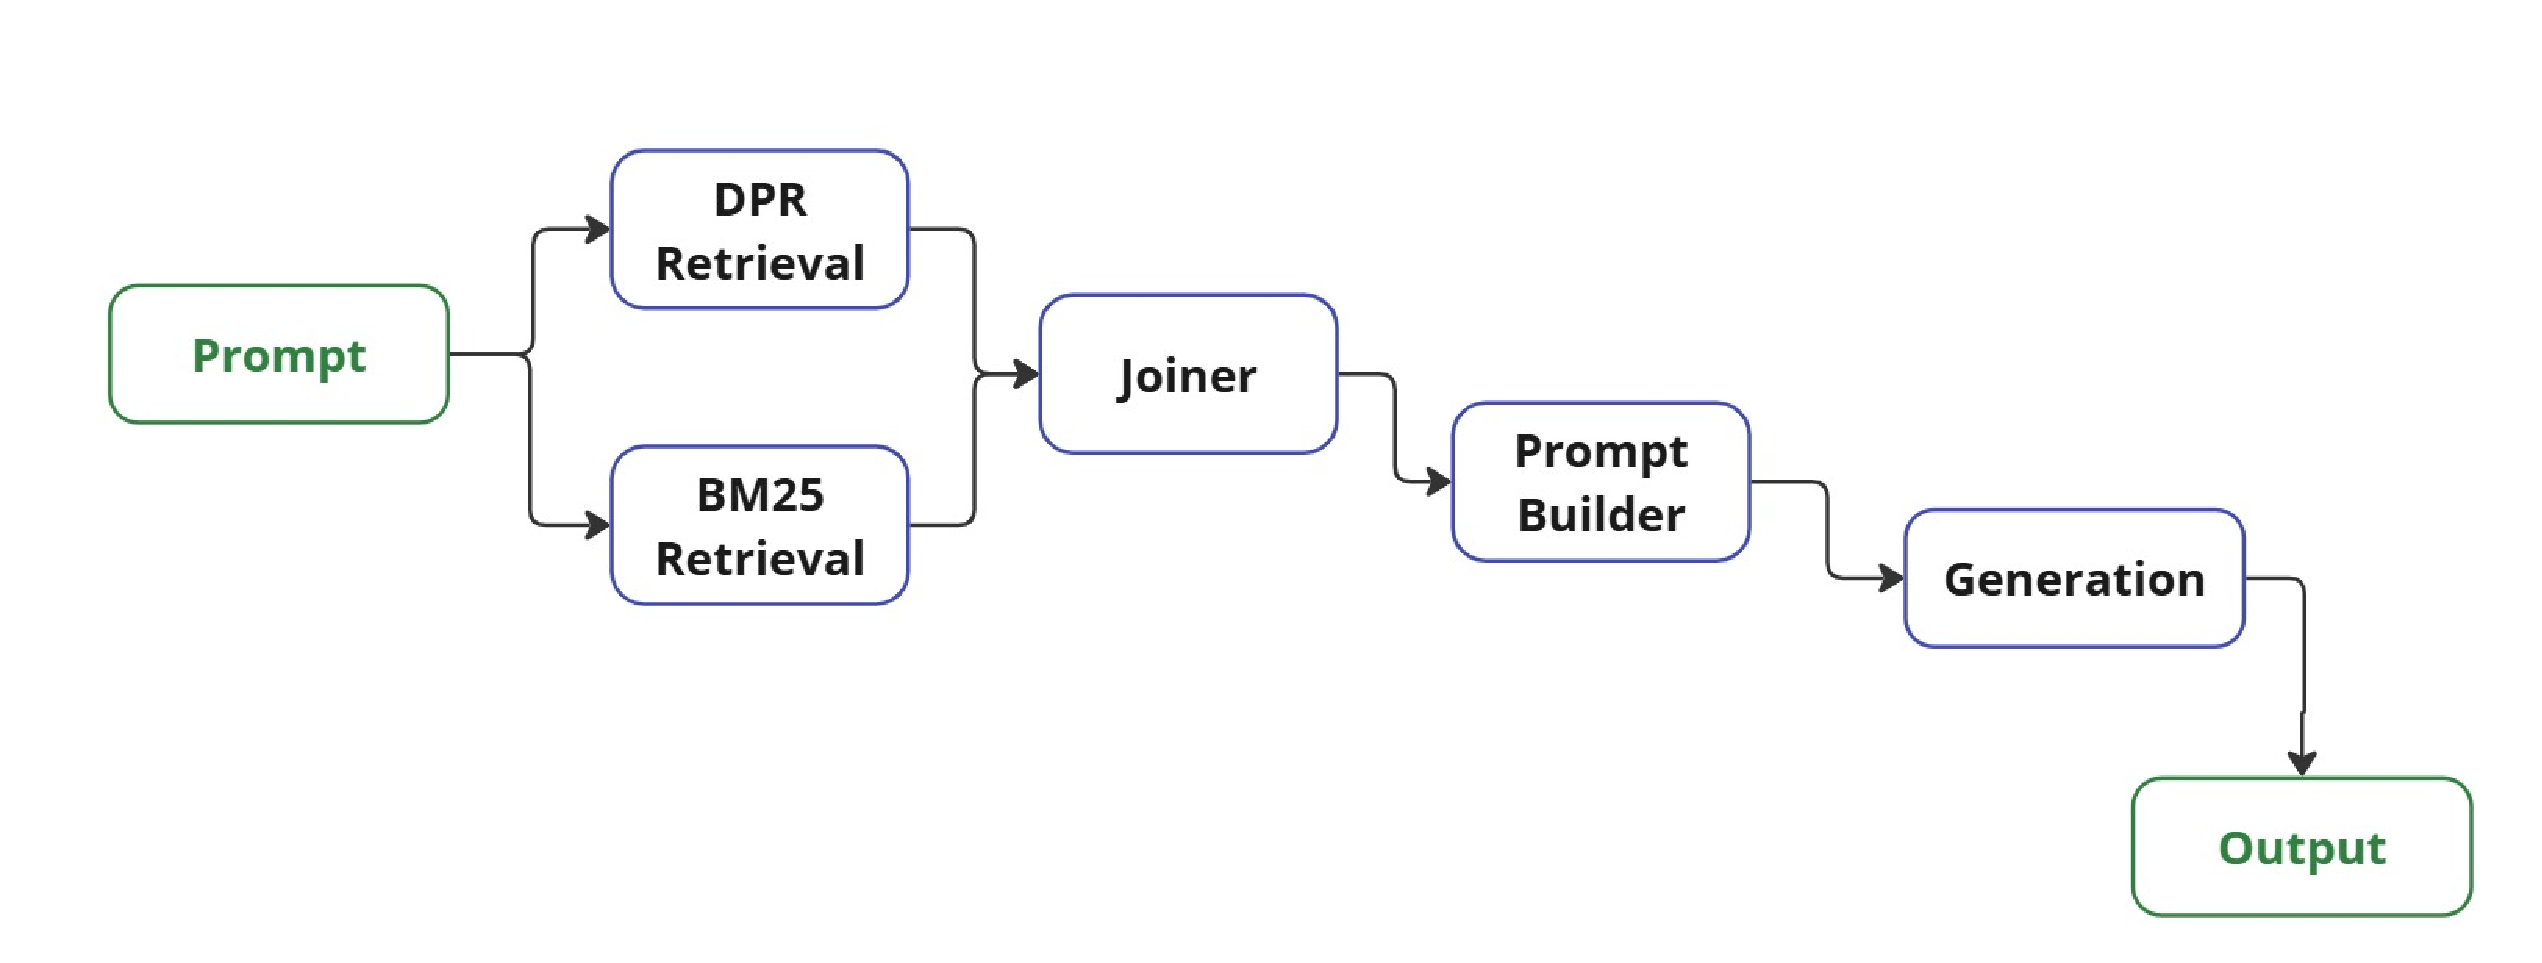
\includegraphics[width=\textwidth]{images/showcase-pipeline.pdf}
    \caption{A simple Retrieve-Read pipeline with both dense and sparse retrieval, definable via YAML.}
    \label{fig:showcase}
\end{figure}

RAG systems possess numerous parameters whose optimal settings are often non-obvious. Researchers typically undergo multiple reconfiguration phases until the RAG system achieves satisfactory performance. Intuitively, more iterative refinement cycles can lead to better results. Therefore, enabling short feedback cycles and rapid development is crucial; it allows for the evaluation of numerous configurations and facilitates quick identification and mitigation of performance bottlenecks. This section outlines our approach and considerations for enabling faster RAG development cycles.

Several RAG development tools and frameworks exist. Widely used ones include Llama-Index \cite{Liu_LlamaIndex_2022}, Langchain \cite{Chase_LangChain_2022}, and Haystack \cite{Pietsch_Haystack_the_end-to-end_2019}. All offer comparable functionality for building advanced RAG systems with a modular architecture, as introduced by Gao et al. \cite{Gao.18.12.2023}. Haystack provides custom components that support new technologies and offers functionality for users to define pipelines via YAML files. This enhances the reconfigurability of these systems, as it involves changing parameters in a single YAML file instead of editing Python files. It also improves the reporting of experimental methodologies: instead of saving a Python script or module for each configuration, only a YAML file describing the tested RAG architecture is stored. An example of this YAML definition can be seen in Figure \ref{fig:showcase} and the YAML code below.

Configuring via YAML files offers additional benefits. First, existing RAG configurations can be copied easily. Second, pipeline definitions can still be created in Python and subsequently saved in the YAML format. Lastly, Haystack is developing a UI \cite{haystack-ui} for RAG system development, which can be used to create complex systems in a two-dimensional space.

\begin{minted}[
    frame=single,
    bgcolor=lightgray
  ]{yaml}
components:
  llm:
    init_parameters:
      api_base_url: null
      api_key:
        env_vars: OPENAI_API_KEY
      ...
  prompt_builder: ...
  bm25_retriever: ...
  embedding_retriever: ...
  joiner: ...
  text_embedder: ...
  docs_embedder: ...
  answer_builder: ...
connections:
- receiver: llm.prompt
  sender: prompt_builder.prompt
- ...
\end{minted}

While copying configuration files and adjusting their parameters is more efficient than handling verbose Python modules, we expanded Haystack's core functionality for saving and loading YAML configurations with matrix notation.
This allows specifying different parameters within a list to generate all possible combinations of that configuration. In the example below, four different combinations can be seen: ("gpt-4o-mini", 5), ("o3-mini", 5), ("gpt-4o-mini", 10), and ("o3-mini", 10). This ensures that researchers can test and validate numerous models or parameters and compare their impact on overall performance.

\begin{minted}[
  frame=single,
  bgcolor=lightgray
]{yaml}
components:
  llm:
    init_parameters:
      model: ["gpt-4o-mini", "o3-mini"]
      ...
  retriever:
    init_parameters:
      top-k: [5, 10]
  ...
\end{minted}


Vector databases can differ in functionalities and performance, especially during ingestion. In this framework, we support three different vector databases for experimentation:
\begin{itemize}
  \item In-Memory built-in vector database by Haystack
  \item Chroma vector database \cite{Chroma}
  \item Qdrant vector database \cite{qdrant}
\end{itemize}


\begin{figure}[!ht]
  \centering
  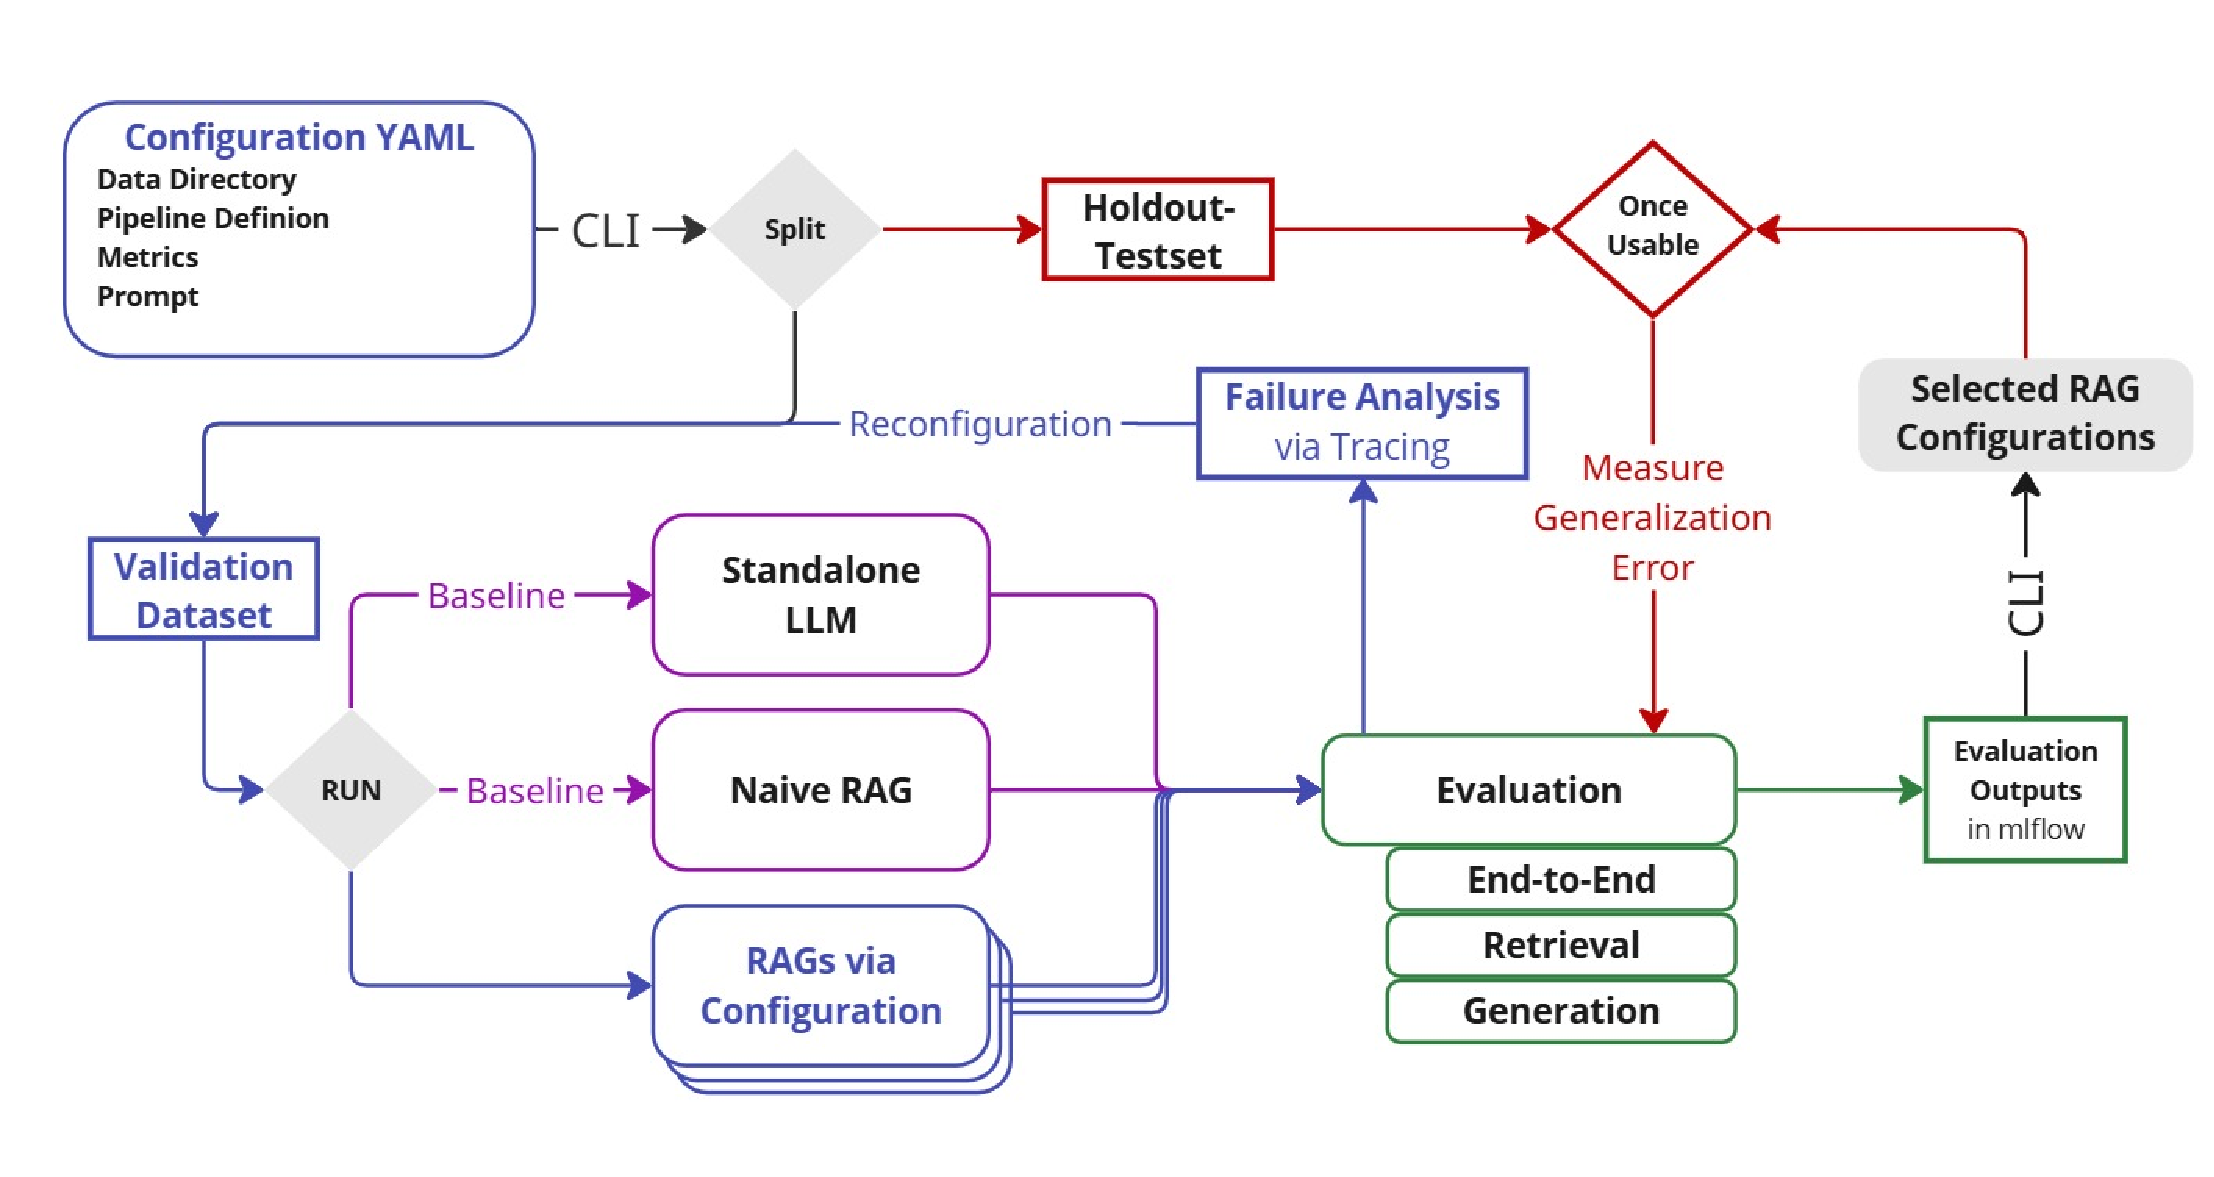
\includegraphics[width=\textwidth]{images/FrameworkFull.pdf}
  \caption{Framework: First, the evaluation data is split into validation and hold-out test datasets. Then, the validation data is used to evaluate a configured RAG system and compare it against baselines. After failure analysis, several reconfiguration phases can occur. Finally, the test dataset is used to test all configurations for potential generalization error.}
  \label{fig:framework-full}
\end{figure}


\section{Transparency}

Following the recommendations of Simon et al. \cite{Simon.10112024} for ensuring transparency in RAG experiments, several practices are crucial. First, transparency requires ensuring that the data used is either publicly available or published alongside the experimental results. While managing data accessibility itself falls outside the direct scope of this framework - typically handled via data repositories or standard version control systems like Git, often hosted on platforms such as GitHub \cite{github-inc-2025} or GitLab \cite{gitlab-inc-2025} - we acknowledge its importance. Data Version Control (DVC) \cite{dvc.17.03.2025} is another popular tool, primarily focused on traditional machine learning experiments. However, its stage-based workflow can introduce overhead that may hinder the rapid iteration cycles common in RAG development. Additionally, its visualization features are often tailored to epoch-based training, which is less relevant for typical RAG evaluation workflows.

Within our recommended workflow, both the framework code and the RAG system architecture should be version controlled (e.g., using Git) with each commit. This practice ensures that each experimental configuration can be precisely restored and transparently reported.

We facilitate this further by enabling the inclusion of metadata parameters directly within the configuration files, a practice we highly recommend for every configuration phase. Researchers can embed comments, document hypotheses, or record observations within the configuration itself, which can later aid in comparing results across different runs within MLflow. Additionally, this metadata makes the rationale behind specific configuration changes more transparent. The benefits include: first, clarifying the researcher's intent (e.g., targeting retrieval versus context utilization improvements); and second, documenting unsuccessful configurations or hypotheses, which can provide valuable negative results for the wider research community.

\begin{minted}[
  frame=single,
  bgcolor=lightgray
]{yaml}
components:
  ...
connections:
- ...
metadata: 
  comment: "This is a comment"
  hypothesis: "This is a hypothesis"
  seed: 42
\end{minted}

Reproducibility in machine learning often relies on random seeding. This can be complex in RAG systems, as not all components or underlying services may expose seeding capabilities. We demonstrate seeding for OpenAI generator components in our example configurations and emphasize the importance of utilizing seeding wherever component parameters allow.

The transparency measures discussed here - publishing data, versioning code and configurations, embedding metadata, and utilizing seeding - contribute significantly to the reproducibility of RAG experiments conducted using this framework. Our approach primarily assumes a relatively static dataset during an experimental cycle. Handling frequently changing datasets might necessitate integrating tools like DVC, which is currently outside the framework's scope. Besides data stability, full reproducibility depends on the ability to define a seed for all components that include randomness.

\section{Validity}

\paragraph{Internal Validity}
Evaluating semantic correctness in LLM and RAG system outputs often relies on either LLM-as-a-Judge models or lexical overlap metrics such as BLEU or ROUGE, which compare the generated output tokens against a reference ground truth. Such lexical metrics often fail to capture semantic equivalence between outputs that use different wording. While LLM-as-a-Judge approaches often correlate well with human judgment, they are susceptible to issues like preference leakage. Research suggests that LLM judges may exhibit biases, potentially favoring outputs from LLMs similar to themselves \cite{Li.03.02.2025}. This field remains an active area of research. In this framework, our LLM-as-a-Judge metrics (e.g., for Context Relevance) utilize a configurable judge model, defaulting via environment variables to OpenAI's \textit{gpt-4o-mini} \cite{OpenAI_2022}. We actively caution users about this potential bias and provide the flexibility to configure a judge model from a different family than the generator LLM being evaluated, mitigating potential self-preference issues.

\paragraph{External Validity}
Our framework addresses a key aspect of external validity through its mandatory use of a validation-test split. As described previously (Section \ref{sec:valtestsplit}), the evaluation dataset is split, and all system tuning and reconfiguration phases are performed using \textit{only} the validation set. This holds true regardless of whether these phases involve simple parameter tuning or training custom components (like fine-tuning a retriever or generator). The held-out test dataset is used only once at the final stage to estimate the generalization performance of the chosen configurations. Within MLflow, users can easily compare the metrics obtained on the validation set during development against the final metrics calculated on the test set for each experimental run. Significant discrepancies between validation and test performance highlight configurations that may have overfitted to the validation set, failing to generalize well.

\begin{figure}[!ht] 
  \centering
  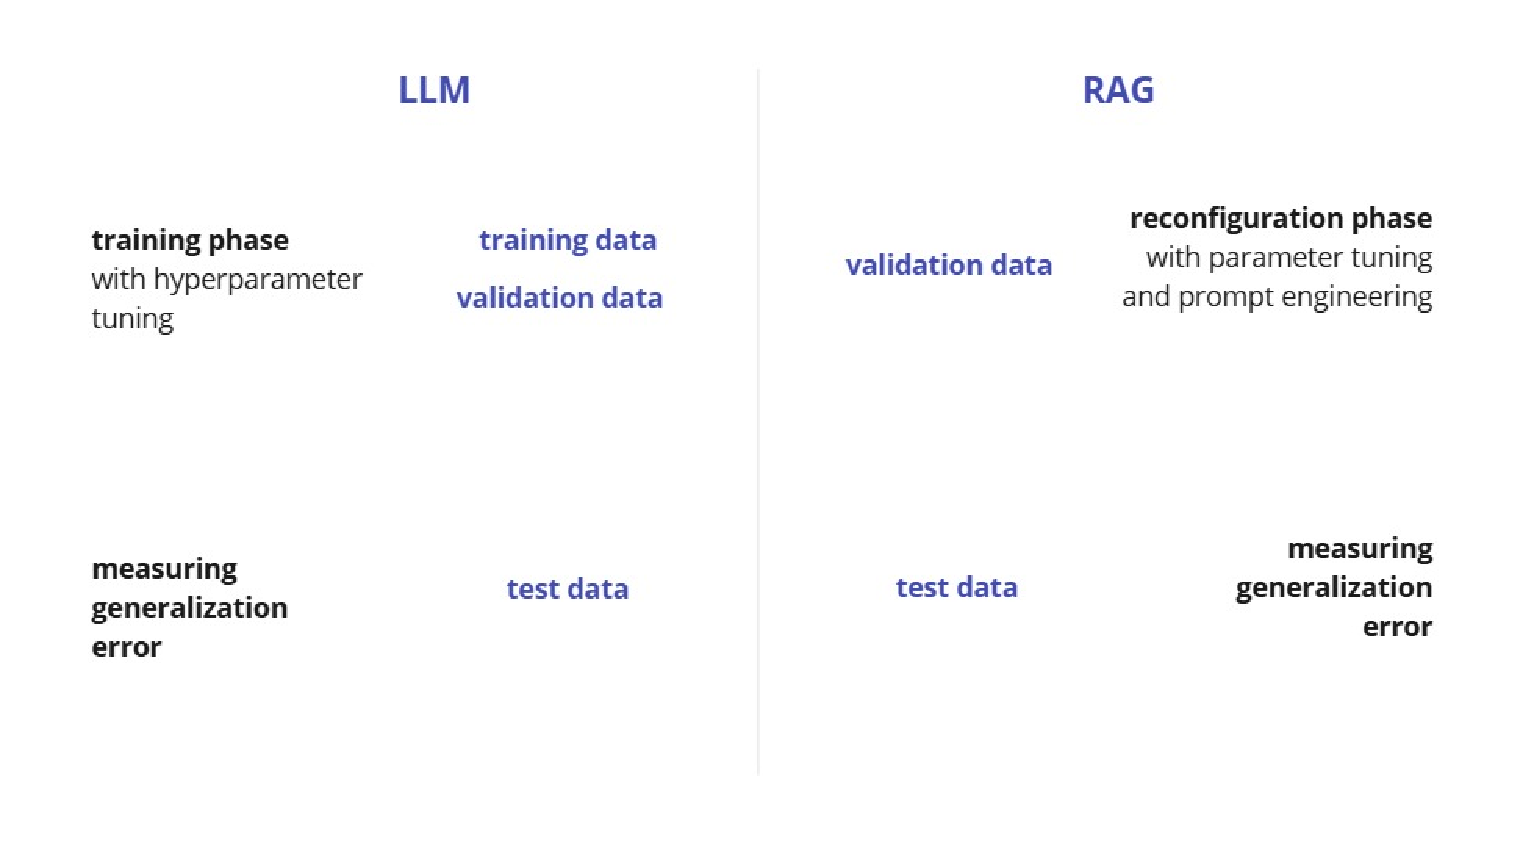
\includegraphics[width=\textwidth]{images/RAGvsLLM-tuning.pdf}
  \caption{Comparison of reconfiguration between RAGs and LLMs - both relying on tuning parameters and test data.}
  \label{fig:tuning}
\end{figure}

\section{User Interface}\label{sec:ui}

Leveraging the previously discussed Haystack functionalities (like YAML pipe\-lines), we have developed a Command-Line Interface (CLI)-based evaluation framework. The complete workflow orchestrated by the framework is depicted in figure \ref{fig:framework-full}. Given paths to an evaluation dataset, pipeline configurations, and metric definitions, the framework first splits the dataset into validation and test sets based on the specified \textit{test\_size} parameter. Subsequently, it uses the validation split to conduct the evaluations.

The framework loads the necessary pipeline components and data and begins by evaluating the baselines: first, a standalone LLM (to assess the value of retrieval itself), and second, after ingesting the data into the specified vector database, a naive BM25-based RAG (Retrieve-Read architecture) baseline (to establish a simple RAG performance level). Following the baseline evaluations, the framework executes and evaluates the RAG pipeline(s) defined in the user-provided YAML configuration file(s). Each evaluated configuration (baselines and user-defined) is assessed using both end-to-end and component-level metrics (as configured). Results (metrics and parameters) are logged to MLflow for visualization and comparison (Figure~\ref{fig:mlflow}), while detailed execution traces are sent to Langfuse for inspection (Figure~\ref{fig:langfuse}). Based on the results and trace analysis, researchers can reconfigure the pipeline YAML and repeat the evaluation process on the validation set.

\begin{figure}[!ht]
  \centering
  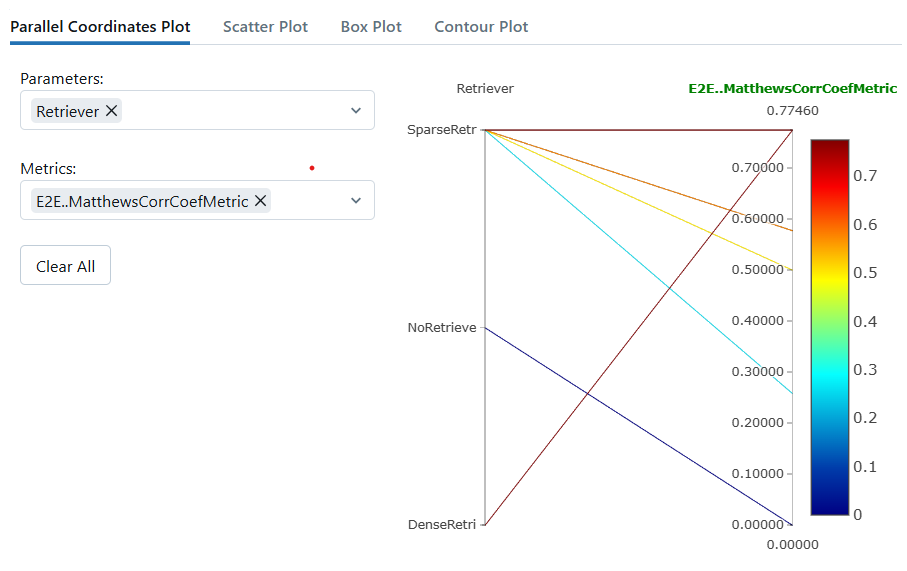
\includegraphics[width=\textwidth]{images/MLFlow-Vis.png}
  \caption{Example of an MLflow run view in our framework. Hypothesis, comments, etc., can be defined via metadata within configuration files. These annotations facilitate comparison and interpretation of results.}
  \label{fig:mlflow}
\end{figure}

\begin{figure}[!ht]
\centering
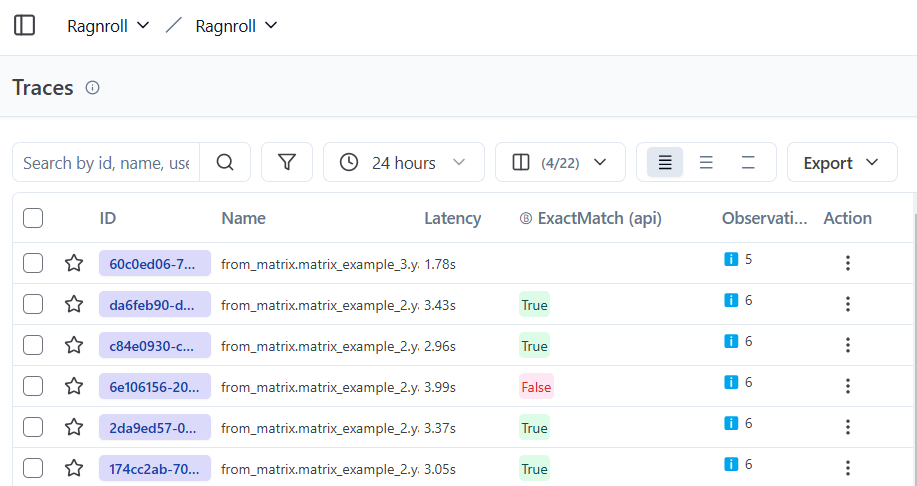
\includegraphics[width=\textwidth]{images/langfuse.png}
\caption{Example Langfuse trace view. Traces log input, output, and intermediate steps for each query, tagged here with success status to aid failure analysis.}
\label{fig:langfuse}
\end{figure}

The framework's CLI, built using Typer, provides commands to streamline the evaluation workflow. The two primary commands are: \texttt{run-evaluations}, which executes the main evaluation loop on the validation set (running baselines and specified YAML configurations); and \texttt{test-generalization}, which runs specified configurations against the held-out test set to assess generalization. Both commands log results and parameters to MLflow and traces to Langfuse. This integration supports efficient, reproducible, and transparent RAG development. The framework is publicly available on GitHub \cite{albrecht-2025}.

\section{Limitations}

The current implementation of this framework primarily focuses on evaluating RAG systems for classification tasks, with built-in support for relevant metrics. However, its design allows for expansion via custom metric implementations, enabling users, in principle, to adapt it for evaluating generative tasks by defining appropriate metric classes.

We implemented the framework to be as modular as possible so that any conceivable architecture with all customized components can be evaluated. However, we cannot guarantee that every architecture is possible, and supporting agentic workflows might require further work.


